\chapter{Differential amplifier with MOS current source}\label{diffampchapter}

\begin{figure}[h]
  \centering
  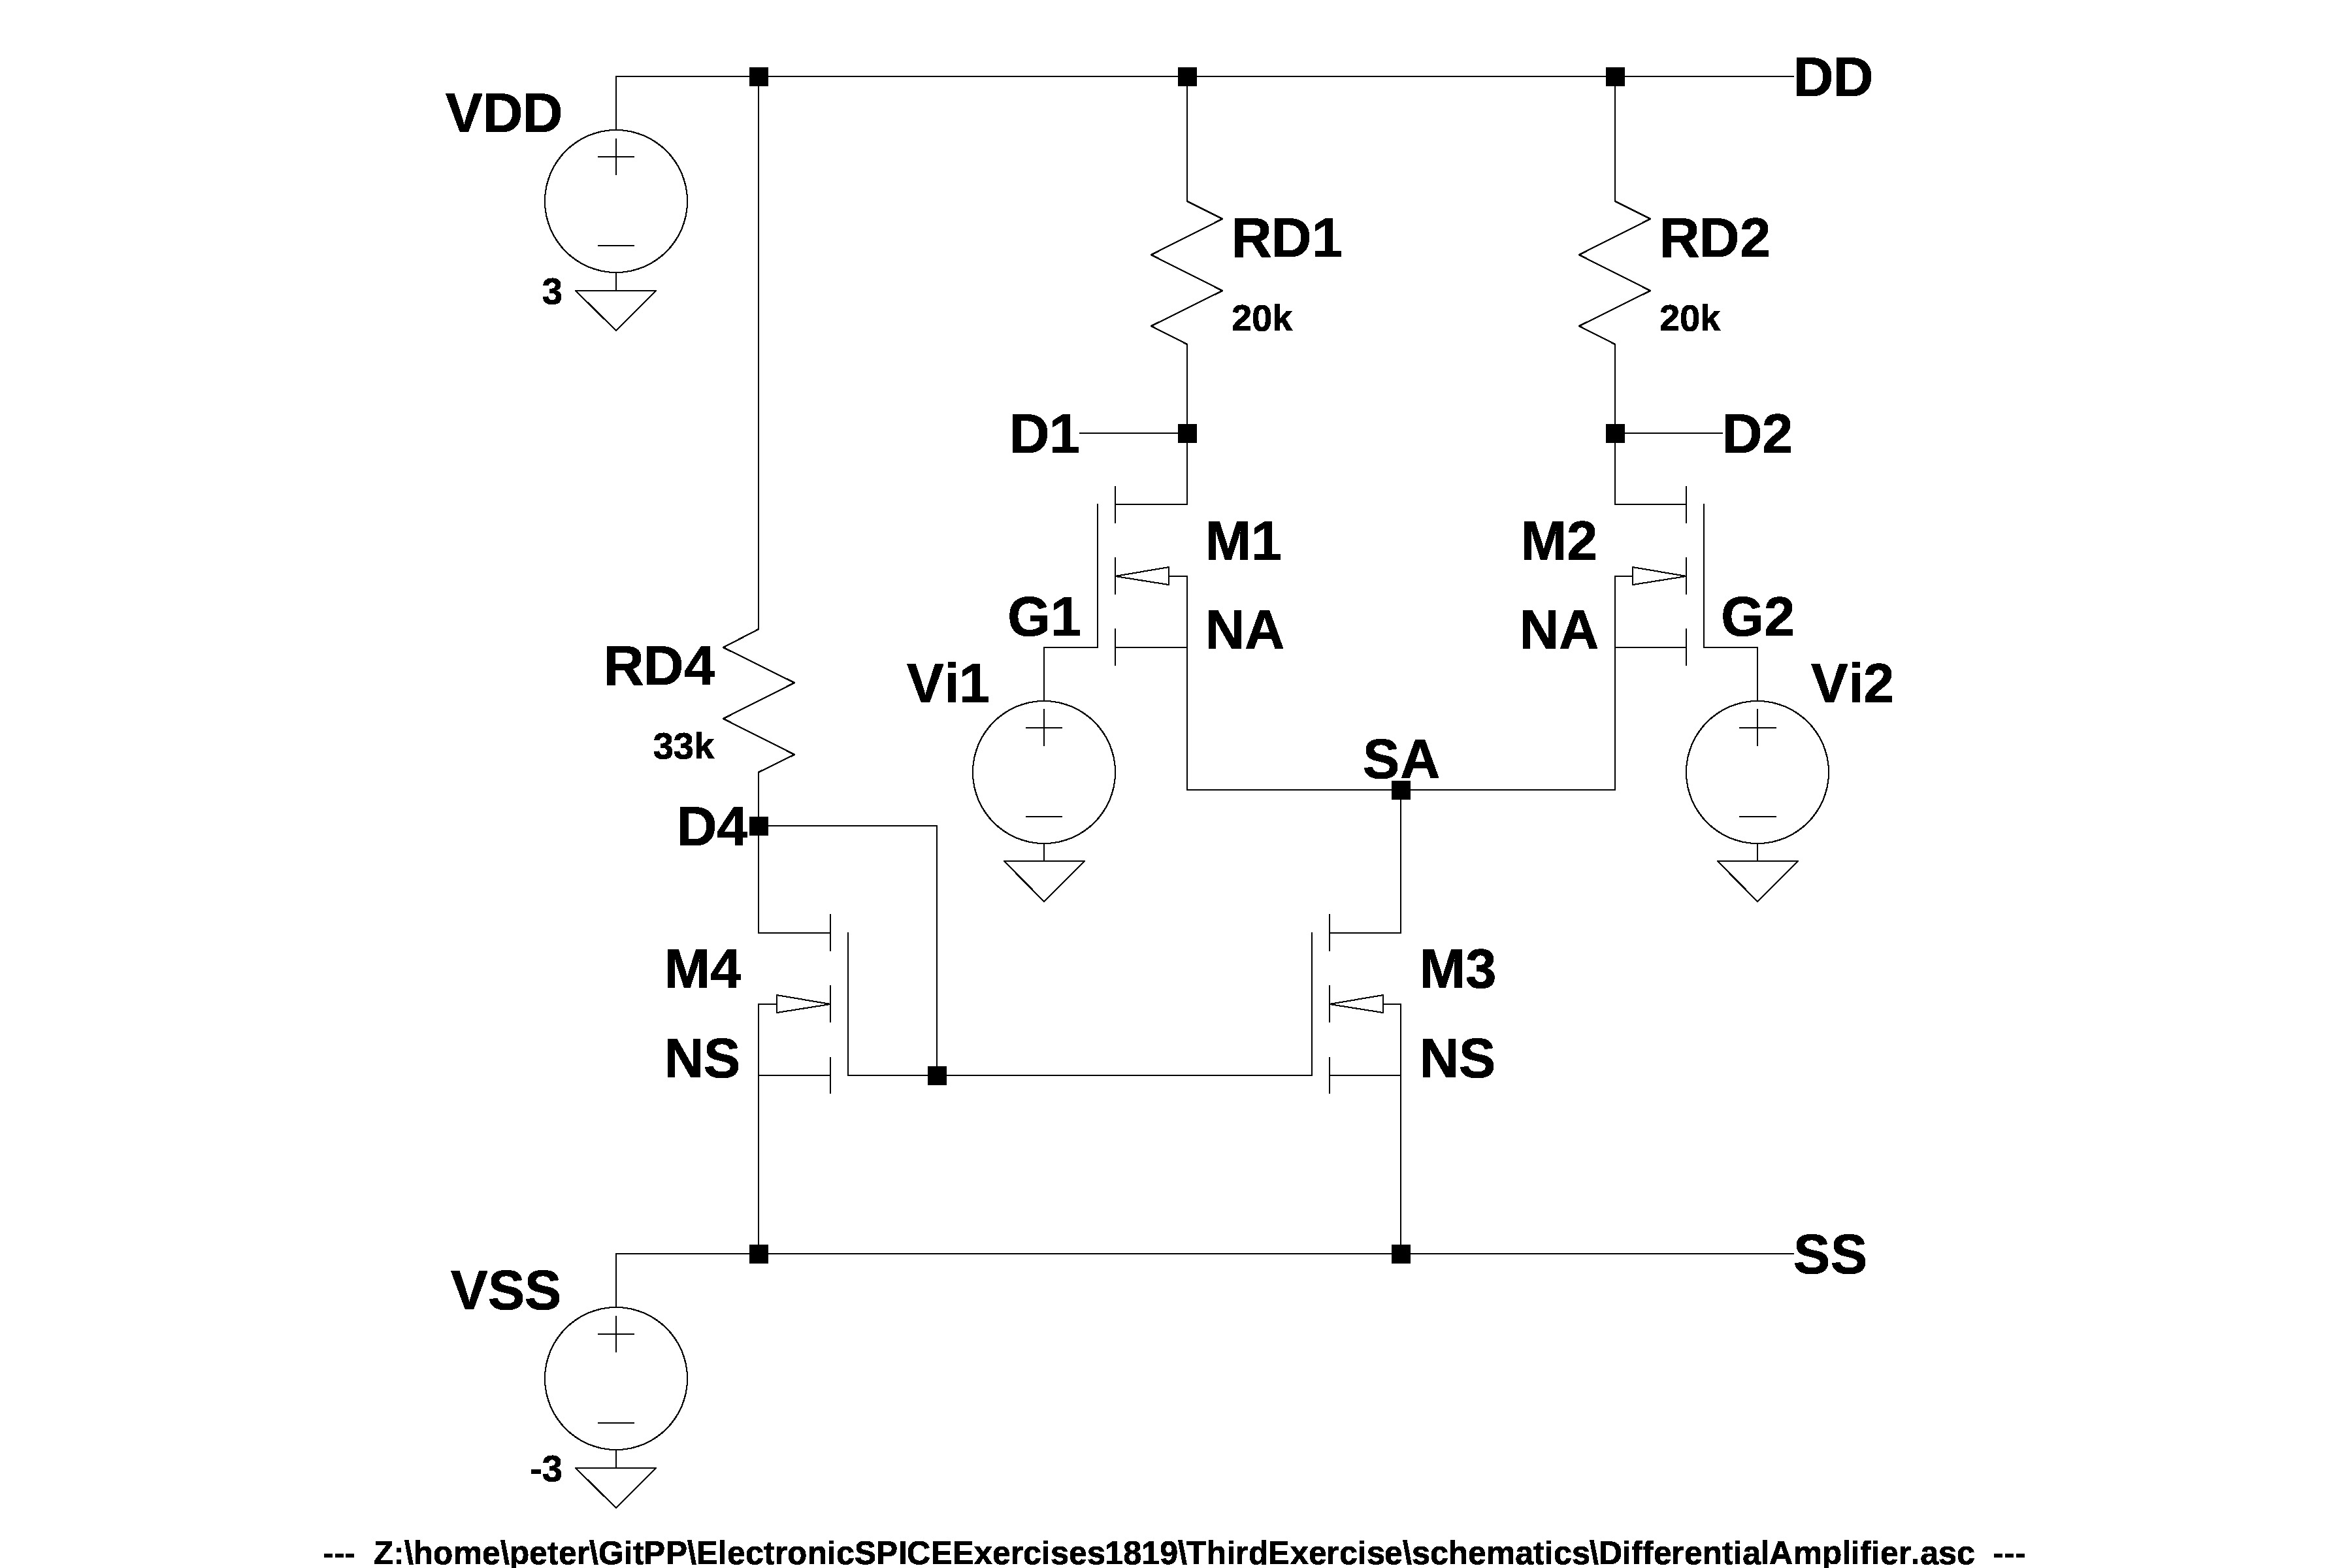
\includegraphics[width=12cm]{schematics/DifferentialAmplifier/Circuit.jpg}
  \caption{Differential amplifier with MOS current source}
  \label{DifferentialAmplifier}
\end{figure}

Initial data:\\
\begin{align}
V_t = 0.5V\\
{K'}_n = {\mu}_n C_{ox} = 200 \frac{\mu A}{V^2}\\
\lambda = 0\\
\left(\frac{W}{L}\right)_1 = \left(\frac{W}{L}\right)_2 = 20\\
\left(\frac{W}{L}\right)_3 = \left(\frac{W}{L}\right)_4 = 5\\
R_{D_1} = R_{D_2} = R_D = 20k\Omega \label{RD}\\
R_{D_4} = \frac{30}{1000}\cdot 1097752 \Omega = 32.93k\Omega \simeq 33k\Omega\\
V_{DD} = 3V\\
V_{SS} = -3V
\end{align}

\section{Static conditions - Analytic solution}

\begin{figure}[h]
  \centering
  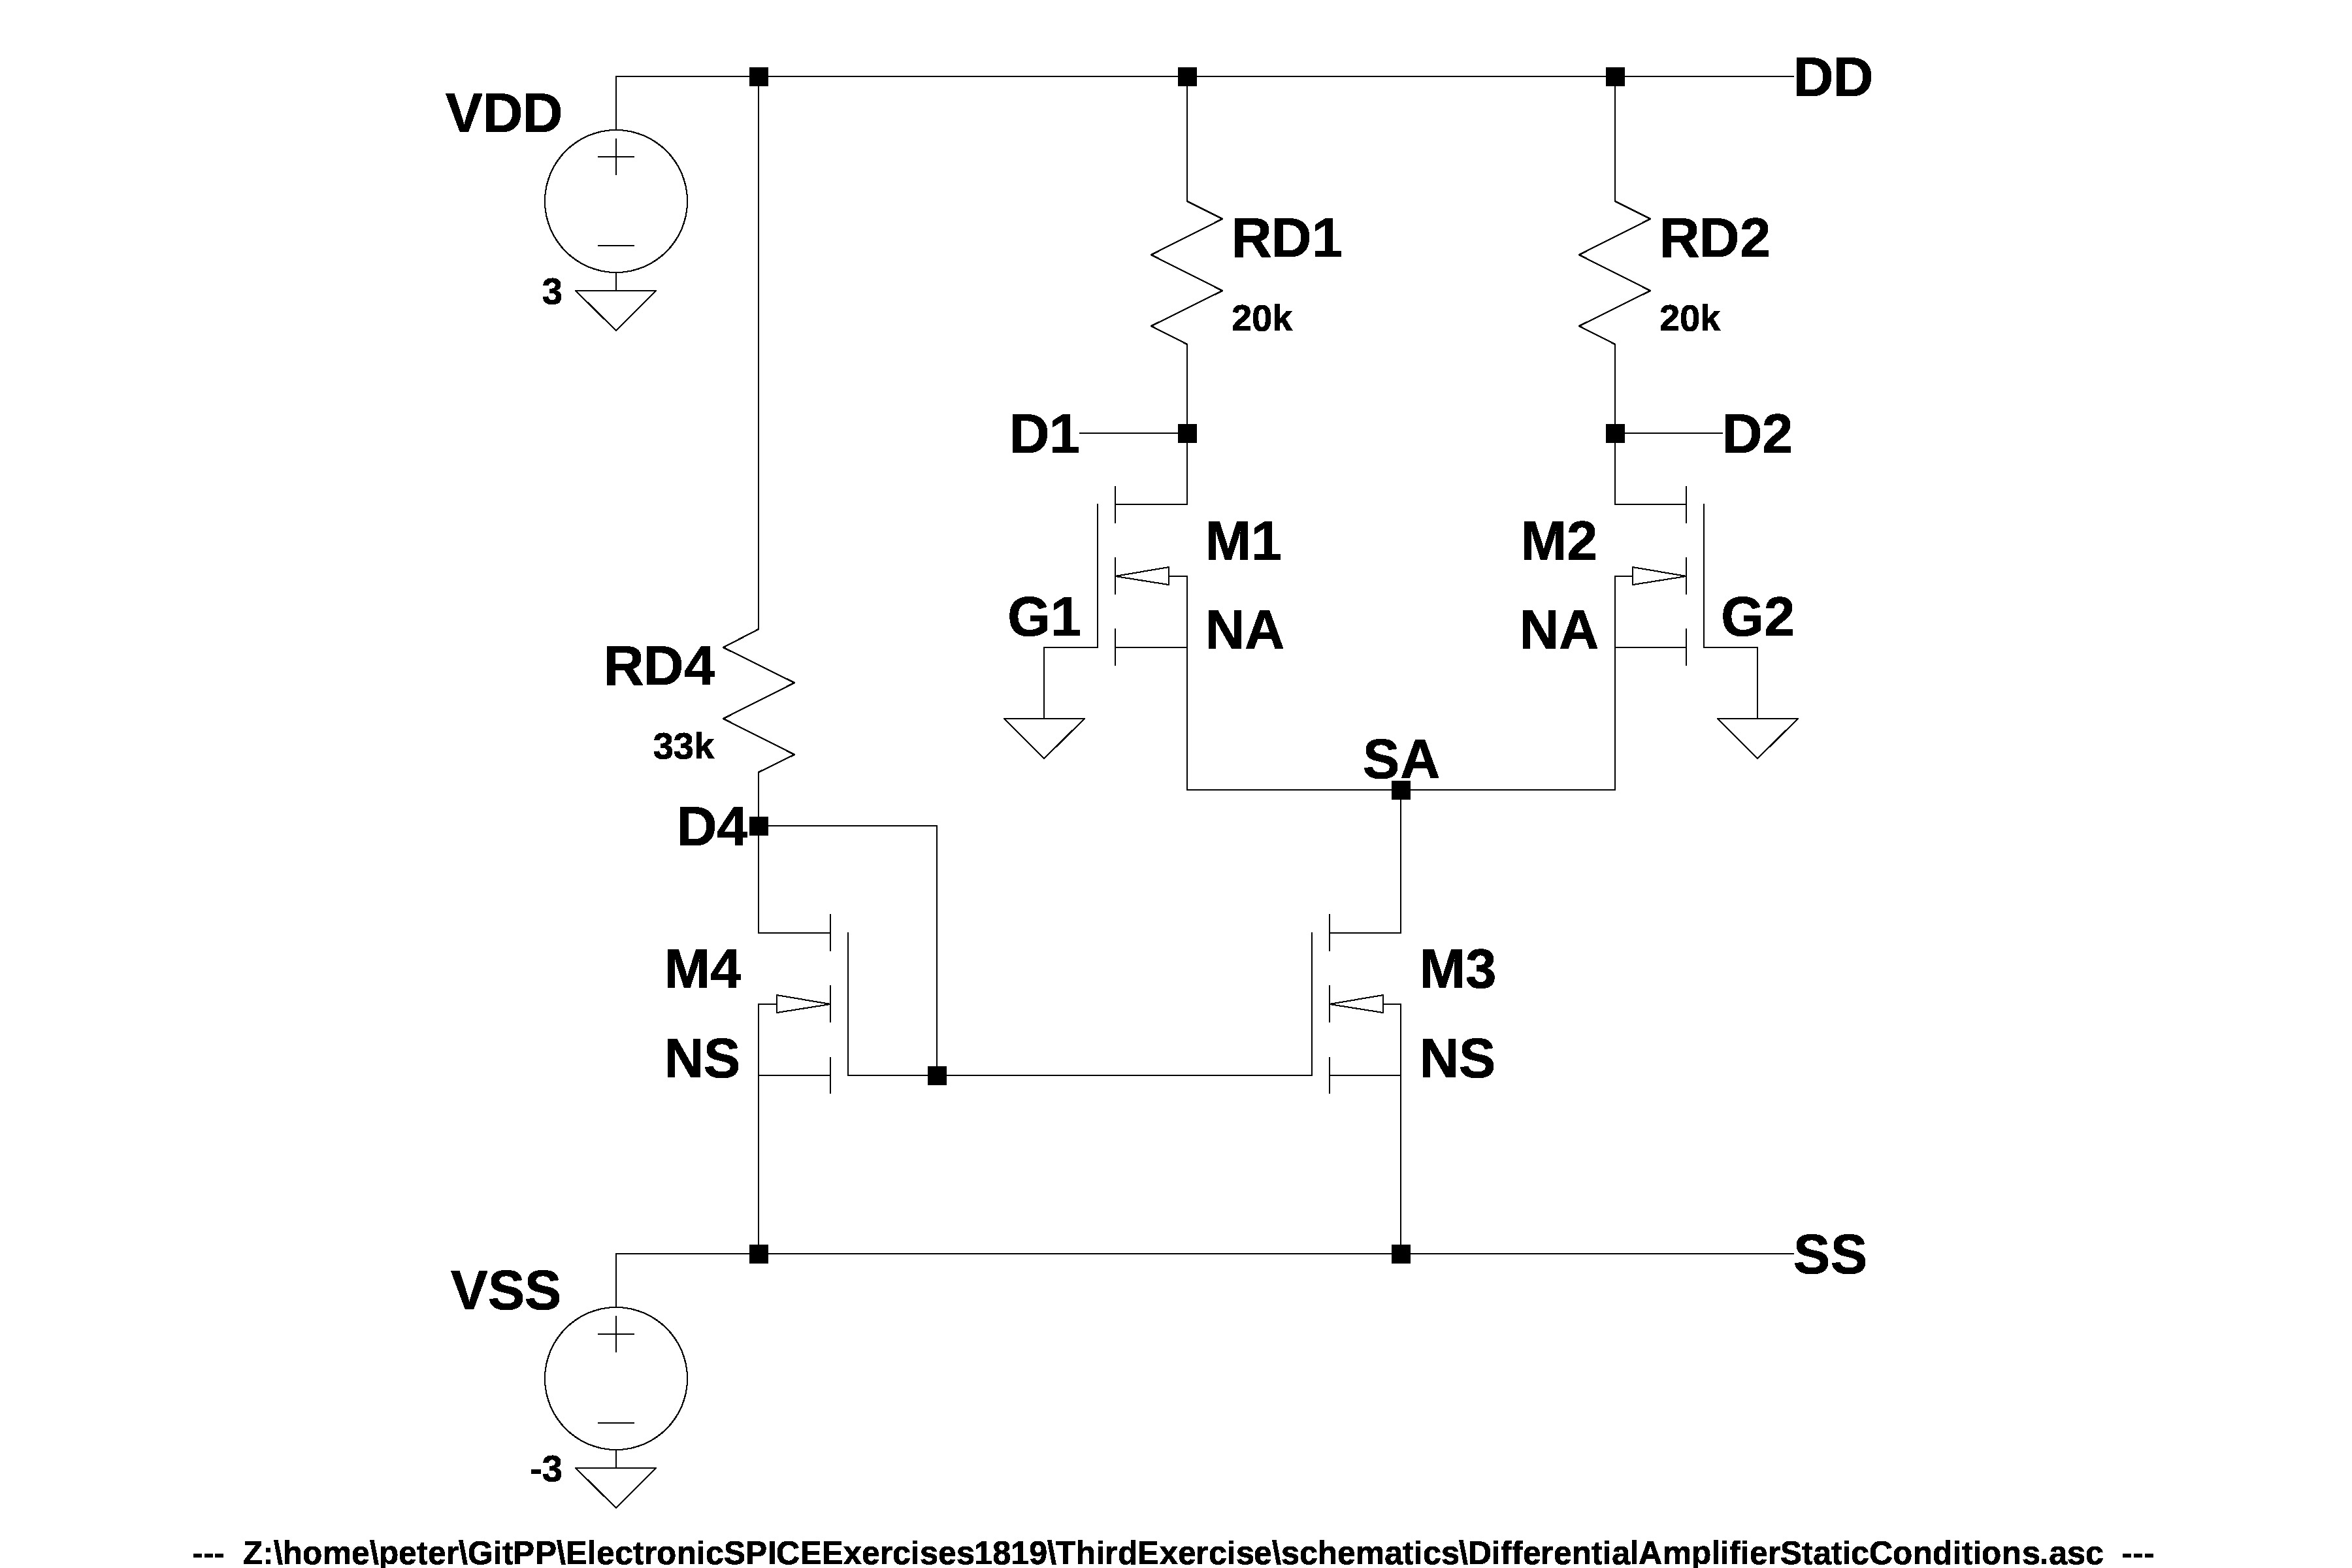
\includegraphics[width=12cm]{schematics/DifferentialAmplifier/StaticConditions.jpg}
  \caption{Differential amplifier with MOS current source - Static conditions}
  \label{DifferentialAmplifierStaticConditions}
\end{figure}

On static conditions it's considered the input signals $V_{i_1}$ and $V_{i_2}$ turned off.\\
The equivalent circuit is on figure \ref{DifferentialAmplifierStaticConditions}.\par

\subsection{MOSFET $M_4$}
\subsubsection{Saturation mode checks}\label{M4SatCheck}
The transistor $M_4$ has a short circuit between its drain and its gate, so the transistor works in saturation mode and the voltage between the drain and the gate are the same of the voltage between the gate and the source:\par
\begin{align}
V_{{D_4}SS} > V_{{G_4}SS} - V_t \xRightarrow{V_{{G_4}SS} = V_{{D_4}SS}}
V_{{D_4}SS} &> V_{{D_4}SS} - V_t\\
0 &> - V_t \quad \text{(Always true: }V_t > 0\text{ )}
\end{align}
It's requested to pay attention to the another check to confirm the work on saturation mode:
\begin{gather}
V_{{G_4}SS} > V_t \xRightarrow{V_{{G4}SS} = V_{{D_4}SS}} V_{{D_4}SS} > V_t \label{CheckSat2eq}
\end{gather}


\subsubsection{$V_{D_4SS}\quad (=V_{G_4SS})$}
Supposing that the transistor $M_4$ works on the saturation mode (see the section \ref{M4SatCheck} for details), the current $I_{D_4}$ could be calculated as:\\
\begin{align}
I_{D_4} &= \frac{1}{2}{K'}_n \left(\frac{W}{L}\right)_4 (V_{D_4SS} - V_t)^2 \label{ID4Sat}
\end{align}
Other expression of the current $I_{D_4}$ could be calculated using the LKT:\\
\begin{align}
V_{DD}-R_{D_4}I_{D_4}-V_{D4SS}-V_{SS} = 0 \implies
I_{D_4} = \frac{V_{DD} - V_{D_4SS} - V_{SS}}{R_{D_4}}\label{ID4K}
\end{align}
Using the equations \ref{ID4Sat} and \ref{ID4K} it's possible calculating $V_{D_4SS}$:\\
\begin{align}
\frac{1}{2}{K'}_n \left(\frac{W}{L}\right)_4 (V_{D_4SS} - V_t)^2 = \frac{V_{DD} - V_{D_4SS} - V_{SS}}{R_{D_4}}
\end{align}
\begin{align}
\frac{1}{2}\cdot 200 \frac{\mu A}{V^2} \cdot 5 \frac{\mu m}{\mu m} (V_{D_4SS} - 0.5V)^2 = \frac{3V - V_{D_4SS} - (-3V)}{33k\Omega}\\
500 \frac{\mu A}{V^2} (V_{D_4SS} -0.5V)^2 = \frac{6}{33}mA-\frac{1}{33k\Omega}V_{D_4SS}\\
500 \frac{\mu A}{V^2} (V_{D_4SS}^2- V_{D_4SS}\cdot V +0.25V^2) = \frac{6}{33}mA-\frac{1}{33k\Omega}V_{D_4SS}\\
500 \frac{\mu A}{V^2} \cdot V_{D_4SS}^2 + \left(-500 \frac{\mu A}{V^2}V + \frac{1}{33k\Omega}\right) V_{D_4SS} + 500 \frac{\mu A}{V^2} \cdot 0.25V^2 -\frac{6}{33}mA = 0\\
0.5 \frac{mA}{V^2} \cdot V_{D_4SS}^2 + \left(-0.5 \frac{mA}{V^2}V + \frac{1}{33k\Omega}\right) V_{D_4SS} + 0.5 \frac{mA}{V^2} \cdot 0.25V^2 -\frac{6}{33}mA = 0\\
\left(0.5 \frac{mA}{V^2}\right) V_{D_4SS}^2 + \left( -\frac{31}{66}\frac{mA}{V}\right) V_{D_4SS} + \left(-\frac{5}{88}mA\right) = 0
\end{align}
\begin{align}
V_{{D_{4}SS}_{1,2}} = \frac{-\left( -\frac{31}{66}\frac{mA}{V}\right)\pm \sqrt{\left(-\frac{31}{66}\frac{mA}{V}\right)^2-4\cdot\left(0.5 \frac{mA}{V^2}\right)\cdot\left(-\frac{5}{88}mA\right)}}{2\cdot0.5 \frac{mA}{V^2}} = 
\left\{
\begin{array}{l}
1.04784V \label{VD4SS}\\
-0.10845V \quad \text{Not possible: }<\text{ of } V_t\\
\end{array}
\right. 
\end{align}

Now it's possible to check the last equation that can confirm the work on saturation mode of the MOSFET $M_4$ (equation \ref{CheckSat2eq}):
\begin{align}
1.04784V > 0.5V \quad M_4 \text{ works on saturation mode.} \label{M4SatConfirm}
\end{align}

\subsubsection{$I_{D_4}$}
Using the equation \ref{ID4Sat} and the result of the equation \ref{VD4SS}:
\begin{align}
I_{D_4} = \frac{1}{2}\cdot 200 \mu A/V^2\cdot 5 \frac{\mu m}{\mu m} \cdot \left(1.04784V -0.5V \right)^2 = 150.06433 \mu A \label{ID4SatResult}
\end{align}

\subsection{MOSFET $M_3$}
\subsubsection{$V_{G_3SS}$}\label{VG3SS}
Observing the circuit represented on the figure \ref{DifferentialAmplifierStaticConditions} it's clear that the voltage $V_{G_3SS}$  is equal to the voltage $V_{D_4SS}$ calculated in the equation \ref{VD4SS}.
\begin{align}
V_{G_3SS} = V_{D_4SS}
\end{align}

\subsubsection{$I_{S_A}$}
As agree with the consideration of the section \ref{VG3SS} and supposing the work of the MOSFET $M_3$ on the saturation mode, it's possible calculating the drain current of the MOSFET $M_3$:\\

\begin{align}
I_{SA} = \frac{1}{2}{K'}_n \left(\frac{W}{L}\right)_3 (V_{D_4SS} - V_t)^2
\end{align}
\begin{align}
I_{SA} = \frac{1}{2}\cdot 200 \mu A/V^2\cdot 5 \frac{\mu m}{\mu m} \cdot \left(1.04784V -0.5V \right)^2 = 150.06433 \mu A \label{ISASat}
\end{align}

\subsubsection{Saturation mode checks}
For obtaining the confirm of the work of the MOSFET $M_3$ on saturation mode the next two equations have to be satisfied:\\
\begin{align}
V_{{D_3}SS} > V_{{G_3}SS} - V_t \xRightarrow{V_{{D_3}SS} = V_{S_ASS}, V_{{G_3}SS} = V_{{D_4}SS}} V_{{S_A}SS} > V_{{D_4}SS} - V_t \label{M3SatCheckVSASS}
\end{align}
\begin{align}
V_{{G_3}SS} > V_t \xRightarrow{V_{{G_3}SS} = V_{{D_4}SS}} V_{{D_4}SS} > V_t \label{M3SatCheckVD4SS}
\end{align}
The equation \ref{M3SatCheckVSASS} hasn't to be checked, $V_{S_ASS}$ isn't calculated yet.\\
The equation \ref{M3SatCheckVD4SS} is satisfied (see the equation \ref{M4SatConfirm}).\par

\subsection{MOSFET $M_1$ and MOSFET $M_2$}
The MOSFET $M_1$ and the MOSFET $M_2$ have the same dimension and the same constructive parameters (see initial data at the start of this chapter \ref{diffampchapter}).\\
They also have the same voltage applied to every their pins (see figure \ref{DifferentialAmplifierStaticConditions}).\\
So, additionally supposing the work on the saturation mode of $M_1$ and $M_2$, it's possible to confirm the next equations:\\
\begin{align}
I_{D_1} &= I_{D_2}\label{ISA/2}\\
V_{G_1S_A} &= V_{G_2S_A}\\
V_{D_1S_A} &= V_{D_2S_A}
\end{align}

\subsubsection{$I_{D_1} (= I_{D_2})$}
\begin{align}
\text{LKC node } S_A \text{: } I_{D_1} + I_{D_2} - I_{S_A} = 0 \xRightarrow{eq. \ref{ISA/2}} 2I_{D_1} - I_{S_A} = 0 \implies I_{D_1} = \frac{I_{S_A}}{2}
\end{align}
\begin{align}
I_{D_1} = \frac{150.06433 \mu A}{2} = 75.03217 \mu A
\end{align}

\subsubsection{$V_{G_1S_A} ( = V_{G_2S_A})$}
Supposing the work of the MOSFET $M_1$ (equally $M_2$) on the saturation mode, the drain current could be calculated as:\\
\begin{align}
I_{D_1} = \frac{1}{2} K'_n \left(\frac{W}{L}\right)_1 (V_{G_1S_A} - V_t)^2 \label{ID1eq}
\end{align}
It's possible using the equation \ref{ID1eq} to calculate $V_{G_1S_A}$:\\
\begin{align}
I_{D_1} &= \frac{1}{2} K'_n \left(\frac{W}{L}\right)_1 (V_{G_1S_A} - V_t)^2\\
\sqrt{I_{D_1}} &= \sqrt{\frac{1}{2} K'_n \left(\frac{W}{L}\right)_1} (V_{G_1S_A} - V_t)\\
\sqrt{\frac{I_{D_1}}{\frac{1}{2} K'_n \left(\frac{W}{L}\right)_1}} &= V_{G_1S_A} - V_t\\
V_{G_1S_A} &= \sqrt{\frac{2I_{D_1}}{K'_n \left(\frac{W}{L}\right)_1}} +V_t\\
V_{G_1S_A} &= \sqrt{\frac{2 \cdot 75.03217 \mu A}{200 \mu A \cdot 20 \frac{\mu A}{\mu A}}} +0.5V\\
V_{G_1S_A} &= 0.69369V \label{VG1SAvalue}
\end{align}

\subparagraph{$V_{S_A}$}
Now it's possible calculating the voltage on the node $S_A$:
\begin{align}
V_{G_1S_A} = V_{G_1} - V_{S_A} \implies V_{S_A} = V_{G_1} - V_{G_1S_A}
\xRightarrow{V_{G_1} = 0, eq. \ref{VG1SAvalue}} V_{S_A} = -0.69369V
\end{align}

\subsubsection{Saturation mode checks}
In order to check the mode of the $M_1$ (and $M_2$) the equations to respect are \ref{M12checkSatA} and \ref{M12checkSatB}.\\
\begin{align}
V_{D_1S_A} &> V_{G_1S_A} - Vt \label{M12checkSatA}\\
V_{D_1} - V_{S_A} &> V_{G_1S_A} - Vt\\
I_{D_1}R_{D_1} - V_{S_A} &> V_{G_1S_A} - Vt\\
75.03217 \mu A \cdot 20k\Omega - (-0.69369V)&> 0.69369V - 0.5V\\
2.19433V &> 0.19369V \quad \text{True.}
\end{align}
\begin{align}
V_{G_1S_A} &> V_t \label{M12checkSatB}\\
0.69369V &> 0.5V \quad \text{True.}
\end{align}


Checking the mode of the $M3$'s work (see equation \ref{M3SatCheckVSASS}):
\begin{align}
V_{{S_A}SS} &> V_{{D_4}SS} - V_t\\
V_{S_A} - V_{SS} &> V_{{D_4}SS} - V_t\\
-0.69369V - (-3V) &> 1.04784V - 0.5V\\
2.30631V &> 0.54784V \quad M_3\text{ works on the saturation mode.}
\end{align}

\subsection{MOSFET $V_{DS_Q}$, $V_{GS_Q}$, $I_{D_Q}$ - Resuming}
\begin{center}
\begin{tabular}{|c|c|c|c|}
\hline
MOSFET & $V_{DS_Q}$ & $V_{GS_Q}$ & $I_{D_Q}$ \\
\hline
$M1$ & $V_{D_1S_A} = 2.19433V$ & $V_{G_1S_A} = 0.69369V$ & $I_{D_1} = 75.03217\mu A$ \\
\hline
$M2$ & $V_{D_2S_A} = 2.19433V$ & $V_{G_2S_A} = 0.69369V$ & $I_{D_2} = 75.03217\mu A$ \\
\hline
$M3$ & $V_{S_ASS} = 2.30631V$ & $V_{D_4SS} = 1.04784V$ & $I_{S_A} = 150.06433 \mu A$ \\
\hline
$M4$ & $V_{D_4SS} = 1.04784V$ & $V_{D_4SS} = 1.04784V$ & $I_{D_4} = 150.06433 \mu A$ \\
\hline
\end{tabular}
\end{center}

\subsection{$g_m$}
\begin{align}
g_{m_1} = g_{m_2} &= K'_n \left(\frac{W}{L}\right)_1 (V_{G_1S_A} - V_t)\\
&= 200 \frac{\mu A}{V^2} \cdot 20 \frac{\mu A}{\mu A} \cdot (0.69369V-0.5V)\\
&= 774.76 \mu A/V
\end{align}
%\begin{align}
%g_{m_3} = g_{m_4} &= K'_n \left(\frac{W}{L}\right)_3 (V_{D_4SS} - V_t)\\
%&= 200 \frac{\mu A}{V^2} \cdot 5 \frac{\mu A}{\mu A} \cdot (1.04784V-0.5V)\\
%&= 547.80 \mu A/V
%\end{align}

\subsection{MOSFET $M_3$ with $\lambda = 0.02$}
From now the MOSFET $M_3$ is considered with $\lambda = 0.02$.\par
On this way there are some changes of the voltages and the currents of the circuit but they could be considered negligible, so it's considered true the past result from now too.\par
With $\lambda = 0.02$, the $r_0$ has a finite value:\\
\begin{align}
r_0 &= \frac{1}{\lambda I_{S_A}}
= \frac{1}{0.02 \cdot 150.06433 \mu A}
\simeq 333.2k\Omega
\end{align}

It's possible see the $r_0$ resitances in the small signal circuit by using the PI model of the transistor MOSFET (figure \ref{PiComplete}).\par

\begin{figure}[h]
  \centering
  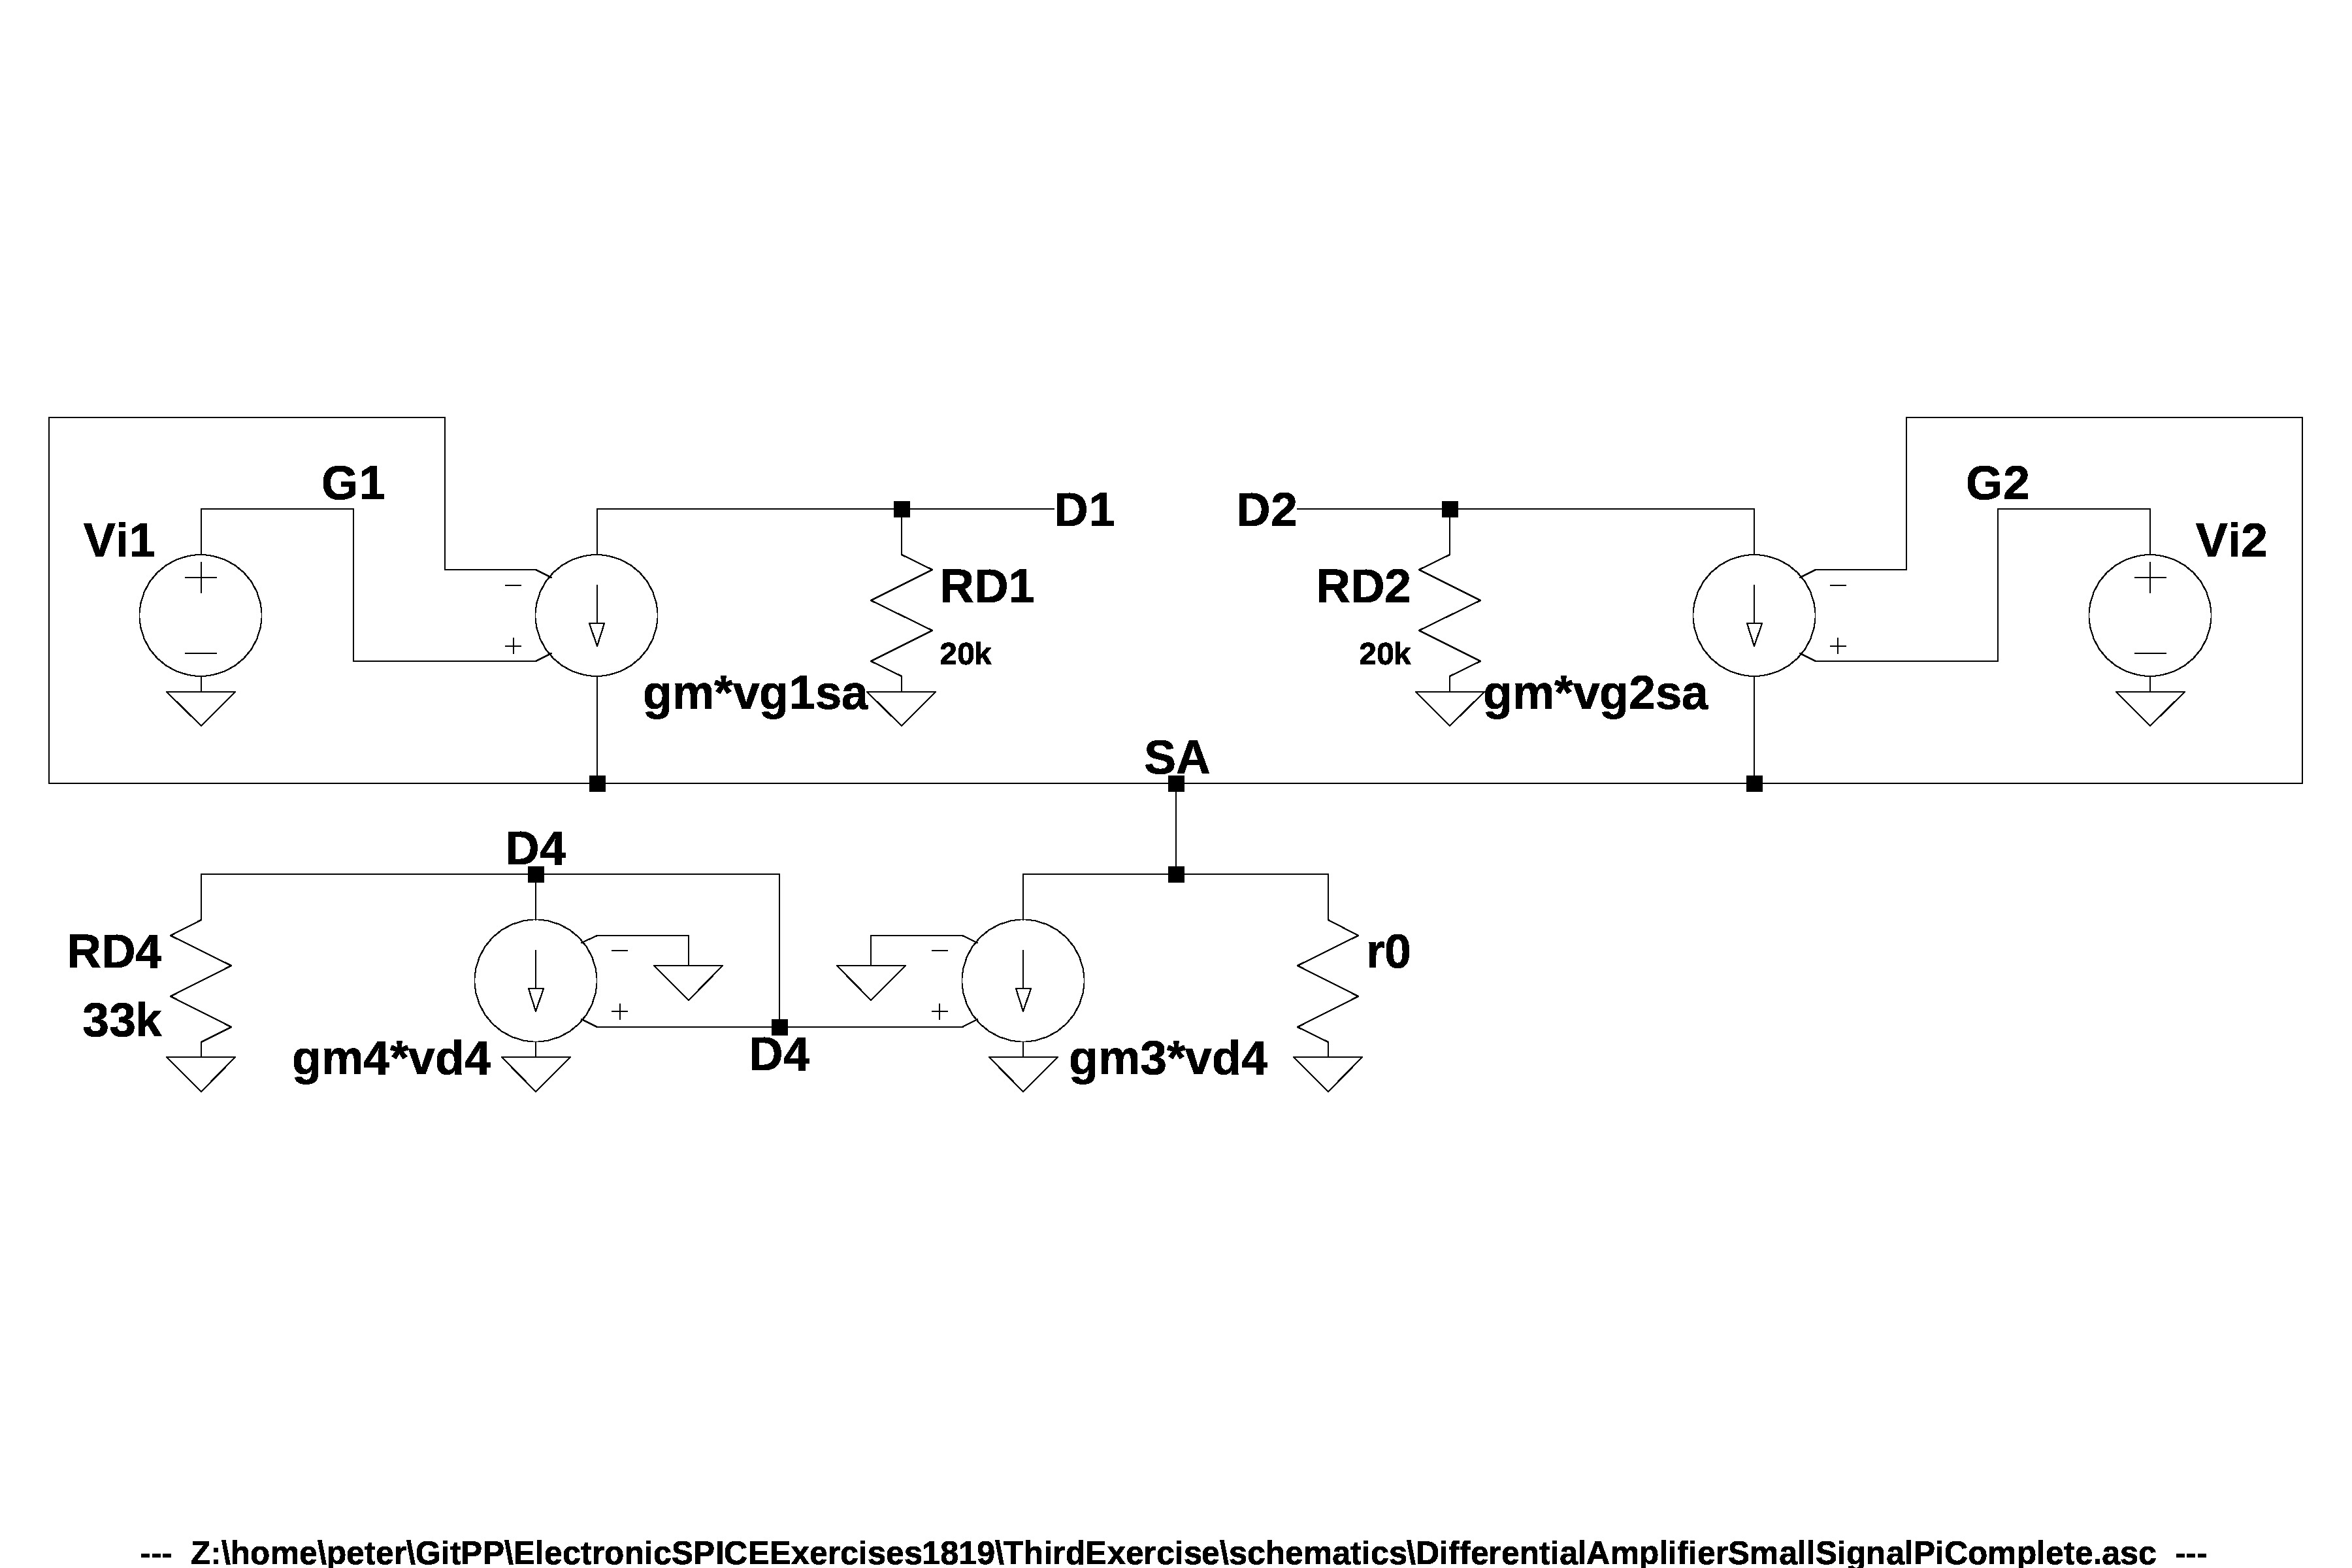
\includegraphics[width=12cm]{schematics/DifferentialAmplifier/SmallSignalPiComplete.jpg}
  \caption{Small signal circuit by using the PI model of the Transistor MOSFET}
  \label{PiComplete}
\end{figure}

In the small signal circuit are considered only the alternate sources, so the $V_{DD}$ and the $V_{SS}$ voltage sources are substituted by a short circuit.\\
In this way the mirror current source composed by the MOSFET $M_4$ and the MOSFET $M_5$ are off because the drain, the source and the gate of these MOSFETs have no voltage applied. So we can simplify the small signal circuit of the figure \ref{PiComplete} to the small signal circuit of the figure \ref{PiSimple}.\par

\begin{figure}[h]
  \centering
  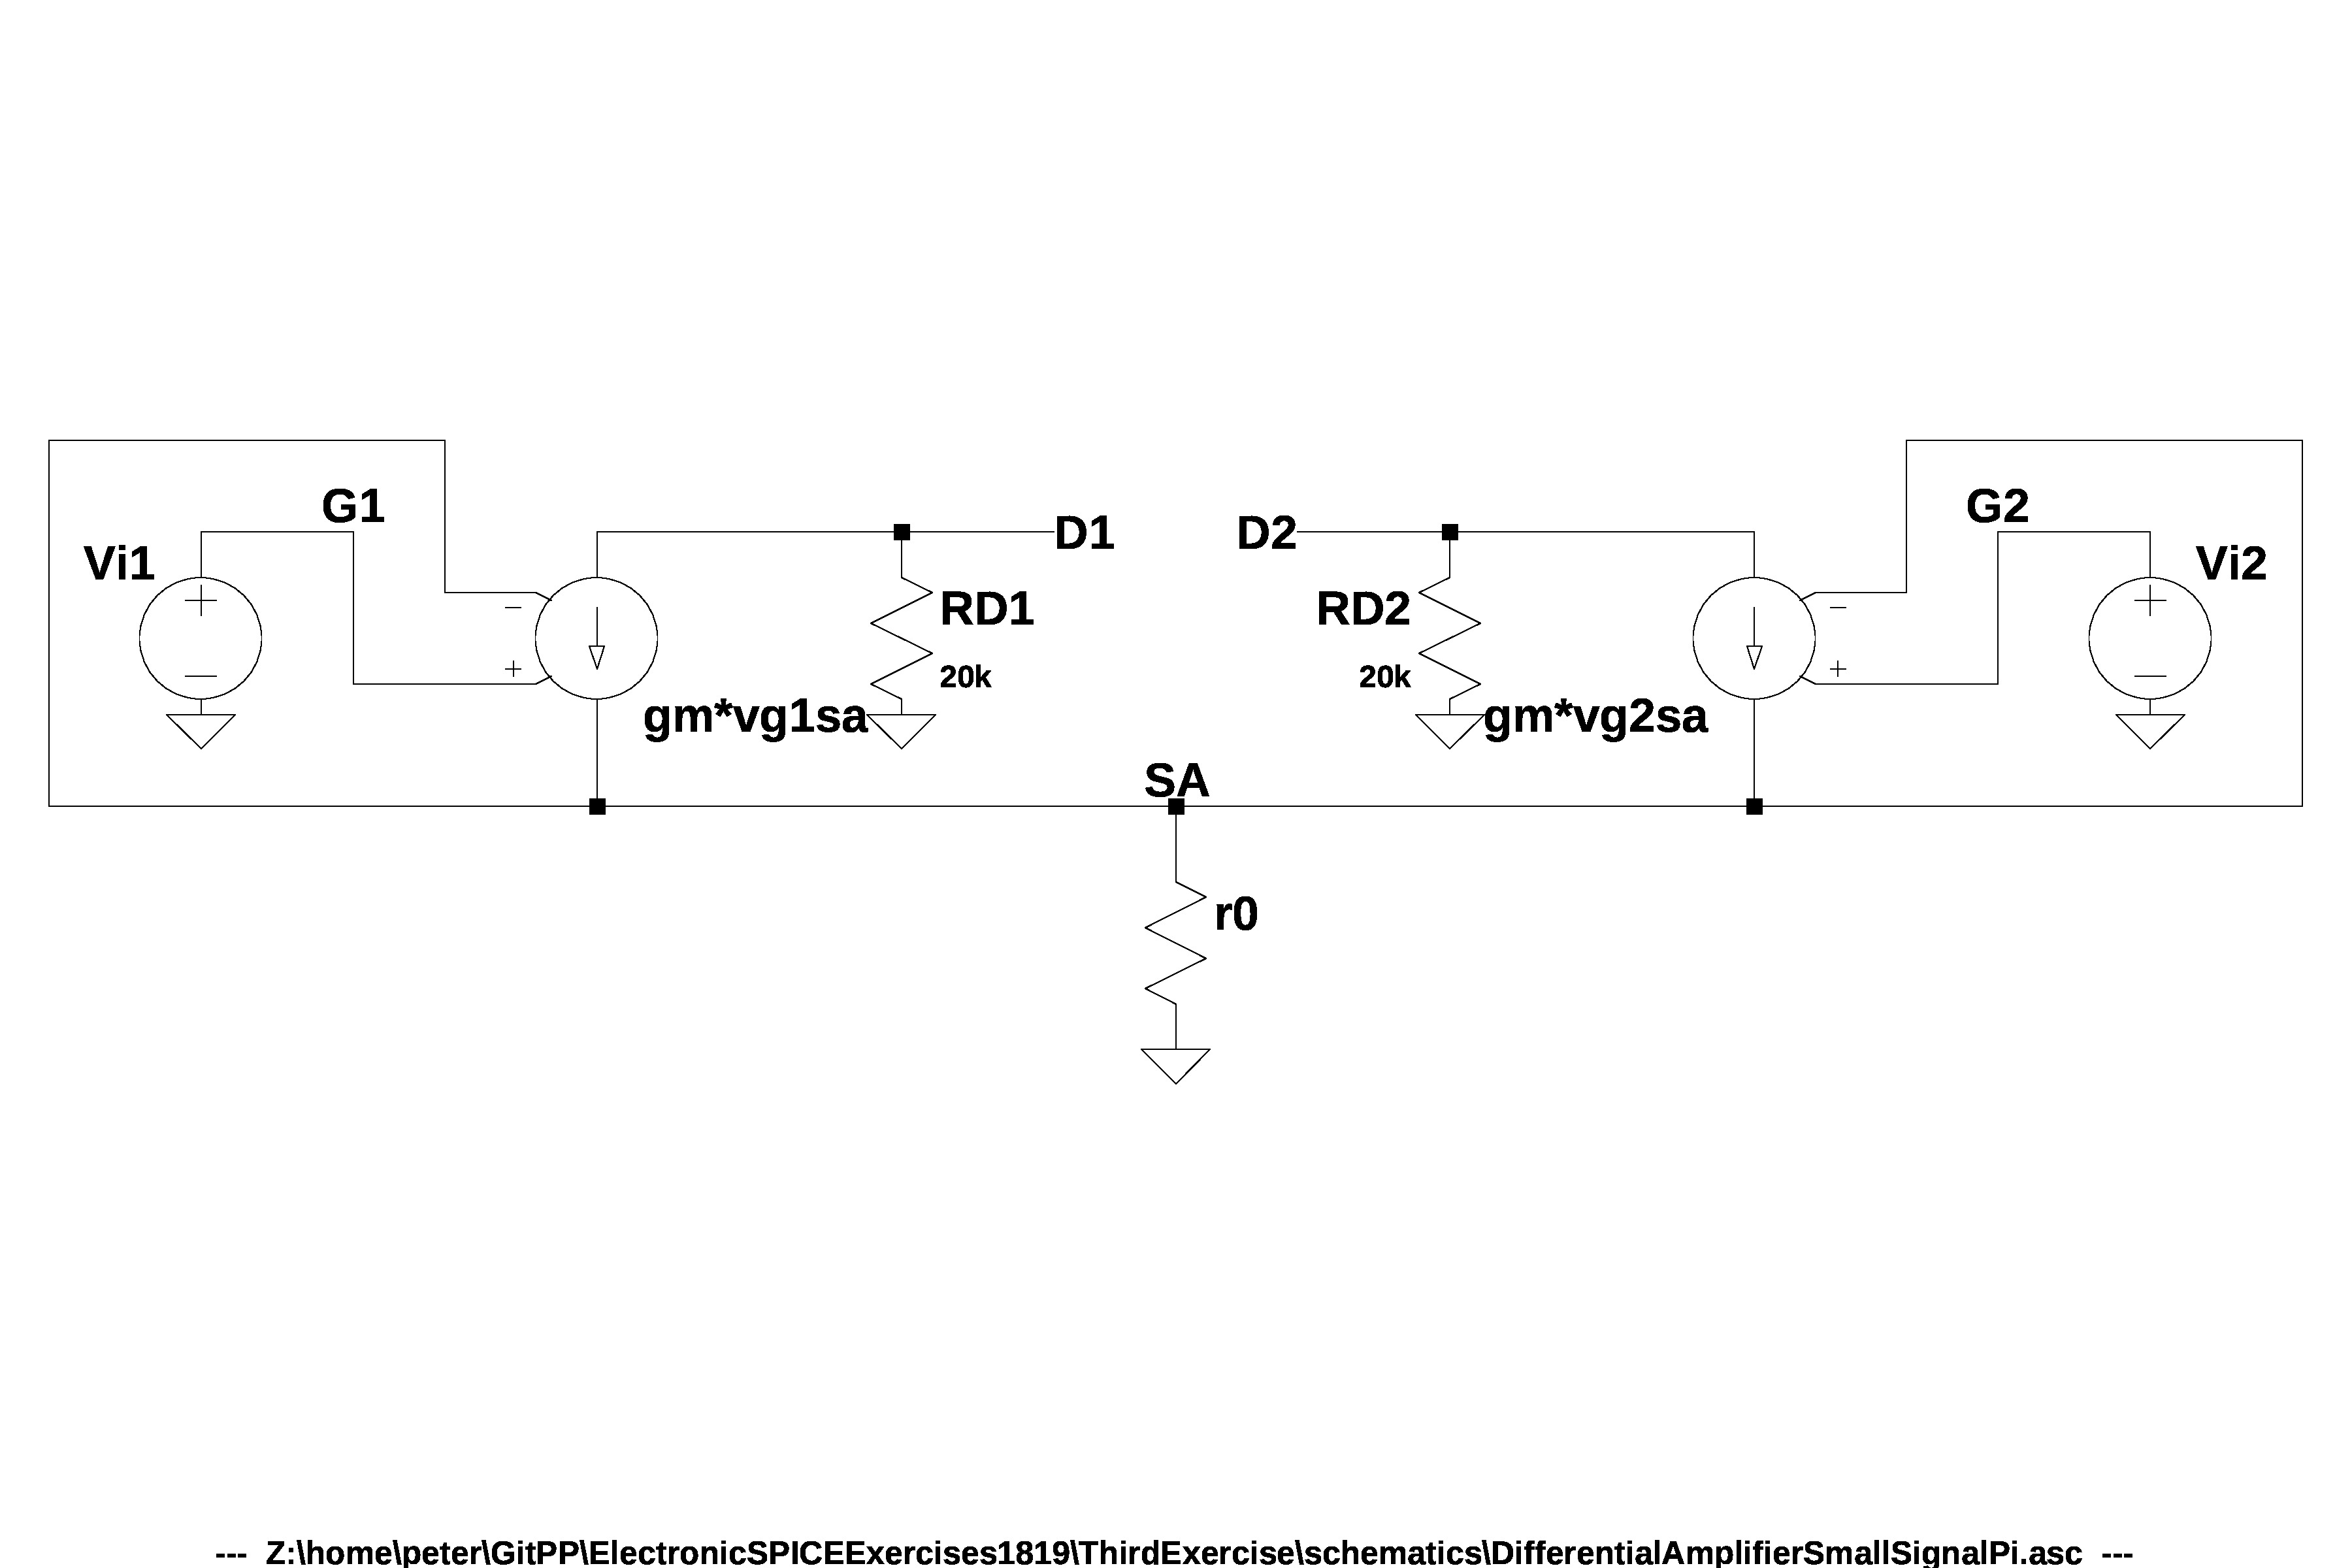
\includegraphics[width=12cm]{schematics/DifferentialAmplifier/SmallSignalPi.jpg}
  \caption{Small signal circuit by using the PI model of the Transistor MOSFET - simplifications}
  \label{PiSimple}
\end{figure}

Now it could be clear the effect of the $\lambda = 0.02$ of the MOSFET $M_3$ because its resistance $r_0$ has an effect to the gain of the circuit if the voltage of the node $S_A$ is different than null.\par

\subsection{Gain single ended}
\subsubsection{Differential pure signal gain}
Now it's applied  small alternate voltage signal to the circuit of the figure \ref{PiSimple}:\\
\begin{align}
V_{i_1} =+ \frac{V_{id}}{2} \label{Vi1d}\\
V_{i_2} =- \frac{V_{id}}{2} \label{Vi2d}
\end{align}


Applying a small alternate voltage signal to the circuit of the figure \ref{PiSimple} the resistance $r_0$ could be treated as a short circuit because the current on it is null.\\
Given that the circuit of the figure \ref{PiSimple} is symmetrical and it's possible analyse the single ended behaviour of the circuit on figure \ref{PiSingle2}.\par

\begin{figure}[h]
  \centering
  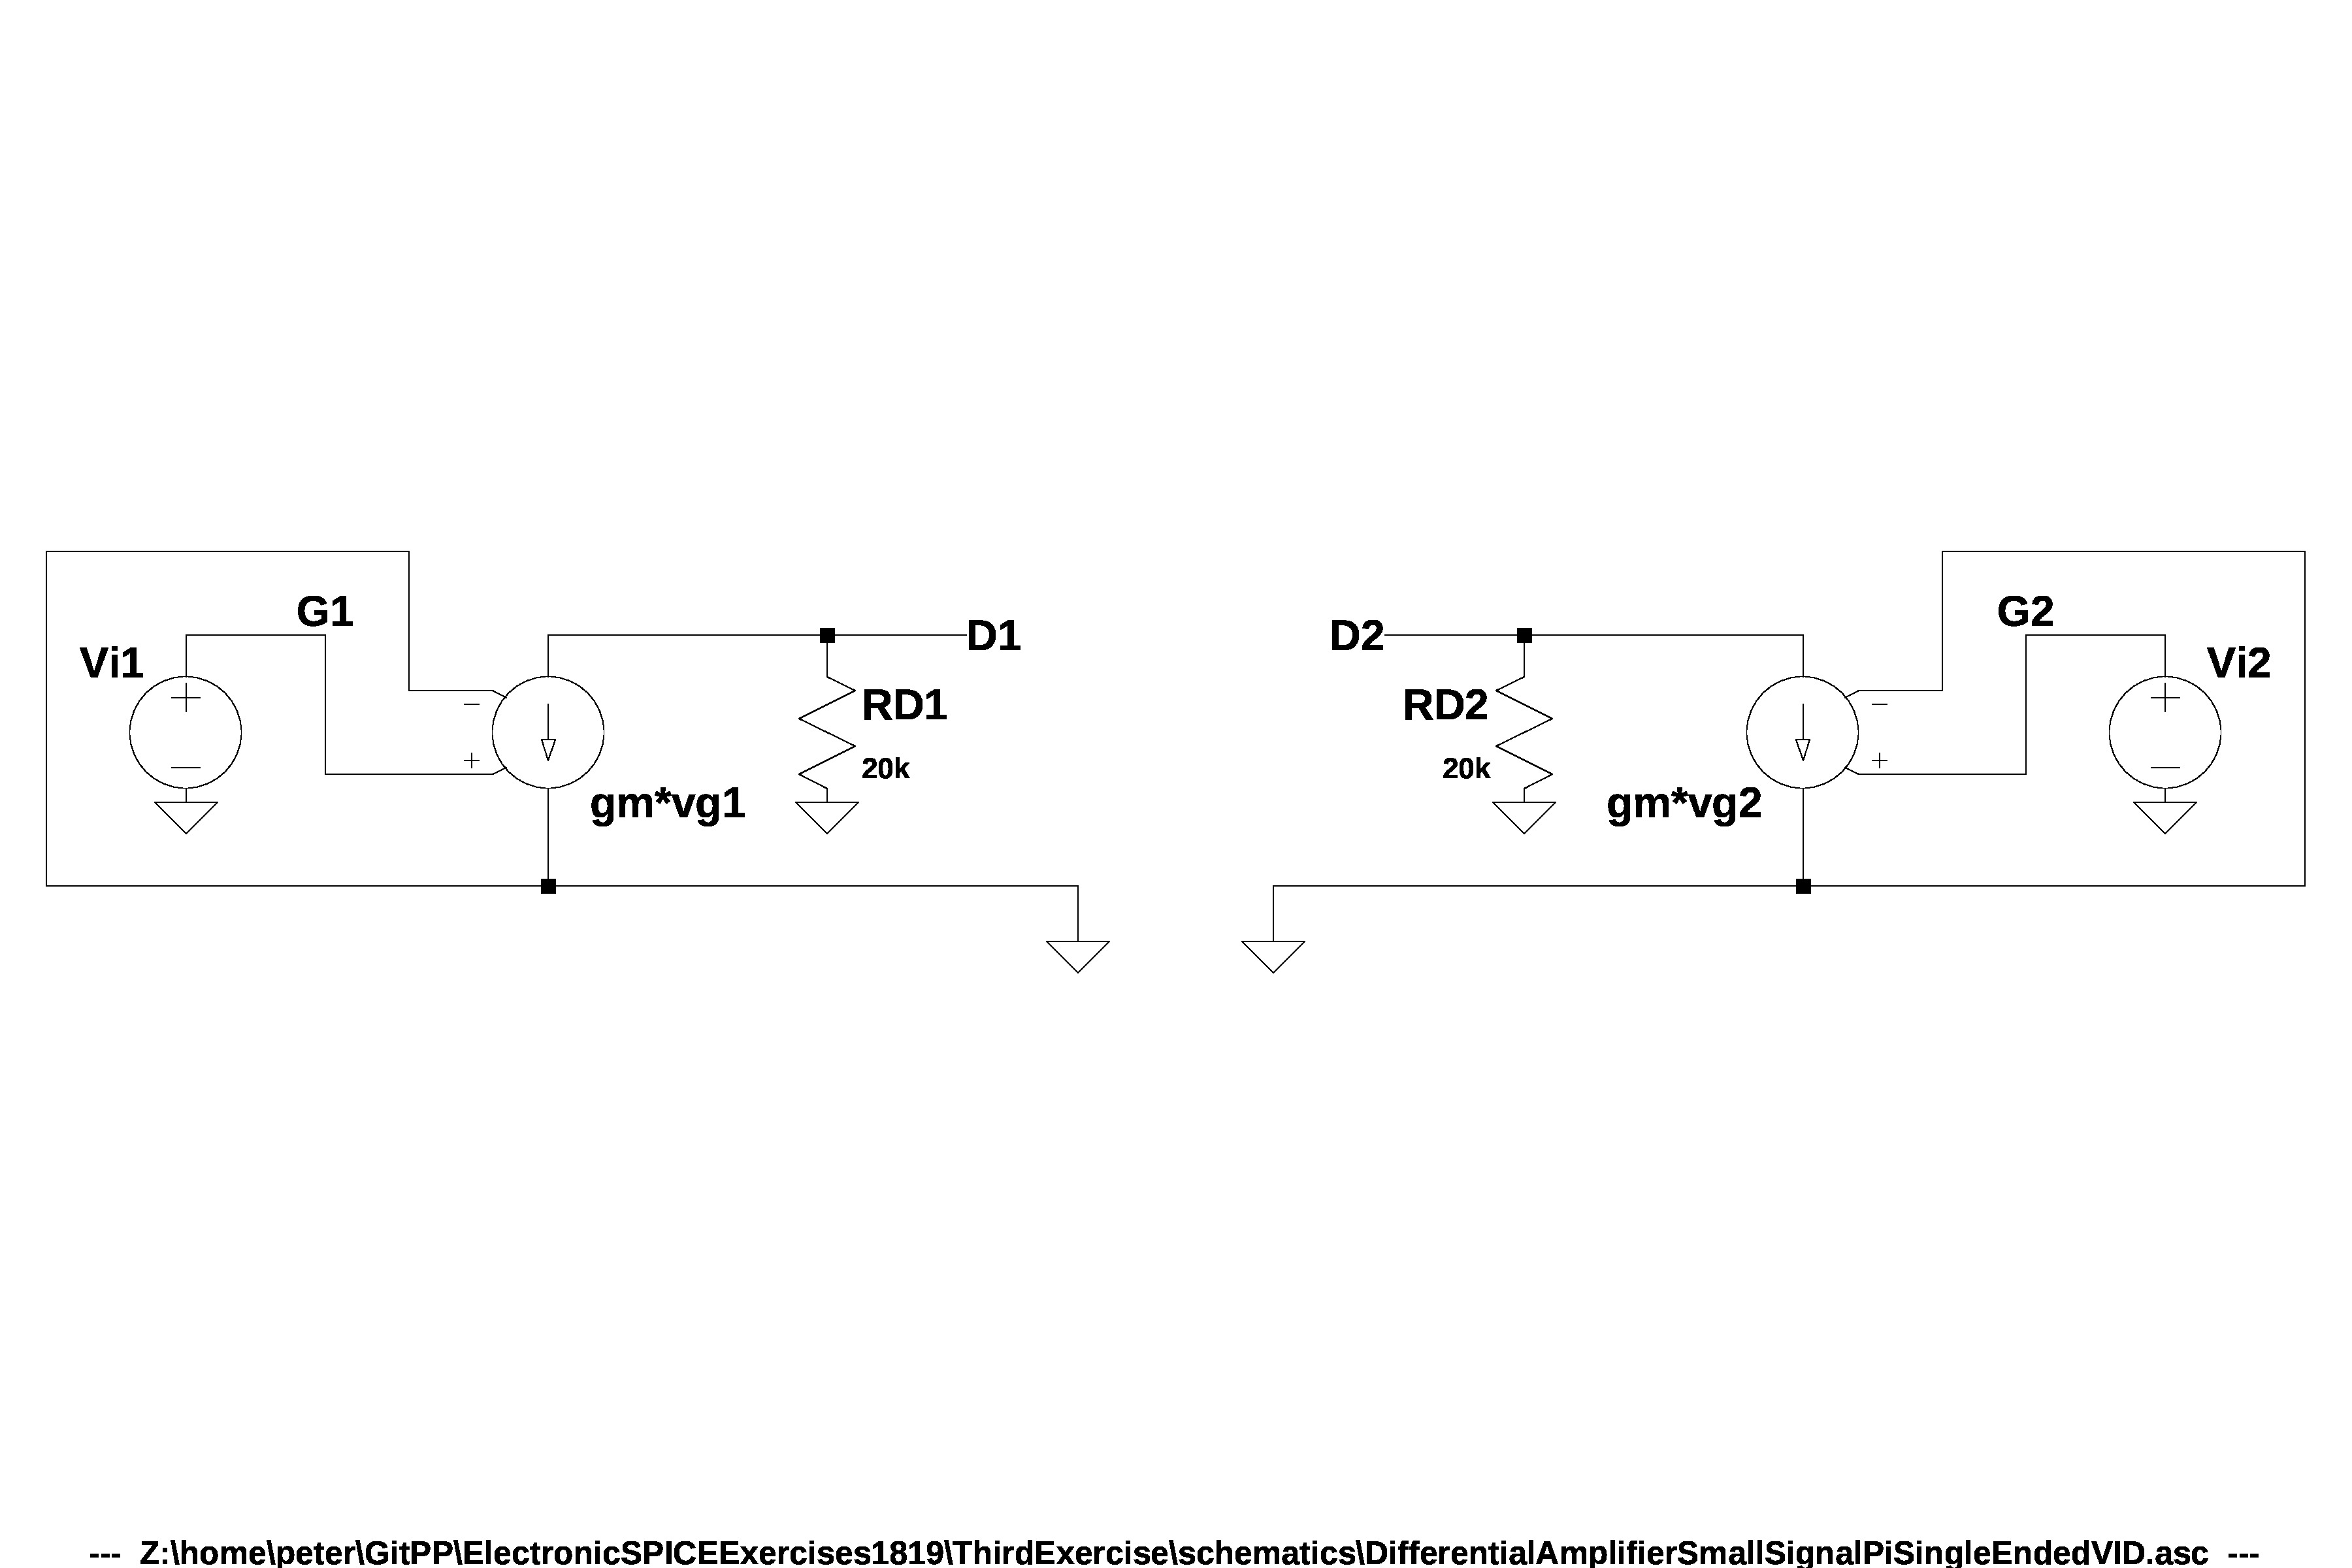
\includegraphics[width=12cm]{schematics/DifferentialAmplifier/SmallSignalPiSingleEndedVID.jpg}
  \caption{Small signal circuit single ended for a differential pure signal.}
  \label{PiSingle2}
\end{figure}

It's possible finding the single ended gain $A_d$ for a small differential signal by calculate first the single ended gain (eq. \ref{Ad1}, \ref{Ad2} and \ref{Ad}).\\

\begin{align}
V_{D_1} = - g_m V_{G_1} R_{D_1} \xRightarrow{(eq. \ref{Vi1d})}
V_{D_2} = - g_m \frac{V_{id}}{2} R_{D_2} \implies
\frac{V_{D_1}}{V_{id}} = - \frac{g_m R_{D_1}}{2} = A_{d_{single\cdot ended\cdot 1}}\label{Ad1}
\end{align}

\begin{align}
V_{D_2} = - g_m V_{G_2} R_{D_2} \xRightarrow{(eq. \ref{Vi2d})}
V_{D_2} = - g_m \left(-\frac{V_{id}}{2}\right) R_{D_2} \implies
\frac{V_{D_2}}{V_{id}} = \frac{g_m R_{D_2}}{2} = A_{d_{single\cdot ended\cdot 2}}\label{Ad2}
\end{align}

\begin{align}
A_d &= \frac{V_{D_2} - V_{D_1}}{V_{id}}\\
&= A_{d_{single\cdot ended\cdot 2}} - A_{d_{single\cdot ended\cdot 1}}\\
&= \frac{g_m R_{D_2}}{2} - \left(- \frac{g_m R_{D_1}}{2} \right)\\
&= \frac{g_m R_{D_2}}{2} + \frac{g_m R_{D_1}}{2}\\
&= \frac{g_m R_{D}}{2} + \frac{g_m R_{D}}{2} \quad \text{(see eq. \ref{RD})}\\
&= g_m R_{D} \label{Ad}
\end{align}

\subsubsection{Common mode gain}
By applying a common mode signal to the inputs of the differential amplifier, on $r0$ there is current different than null, so in this case it gives an important role to the common mode gain.\\
\begin{figure}[h]
  \centering
  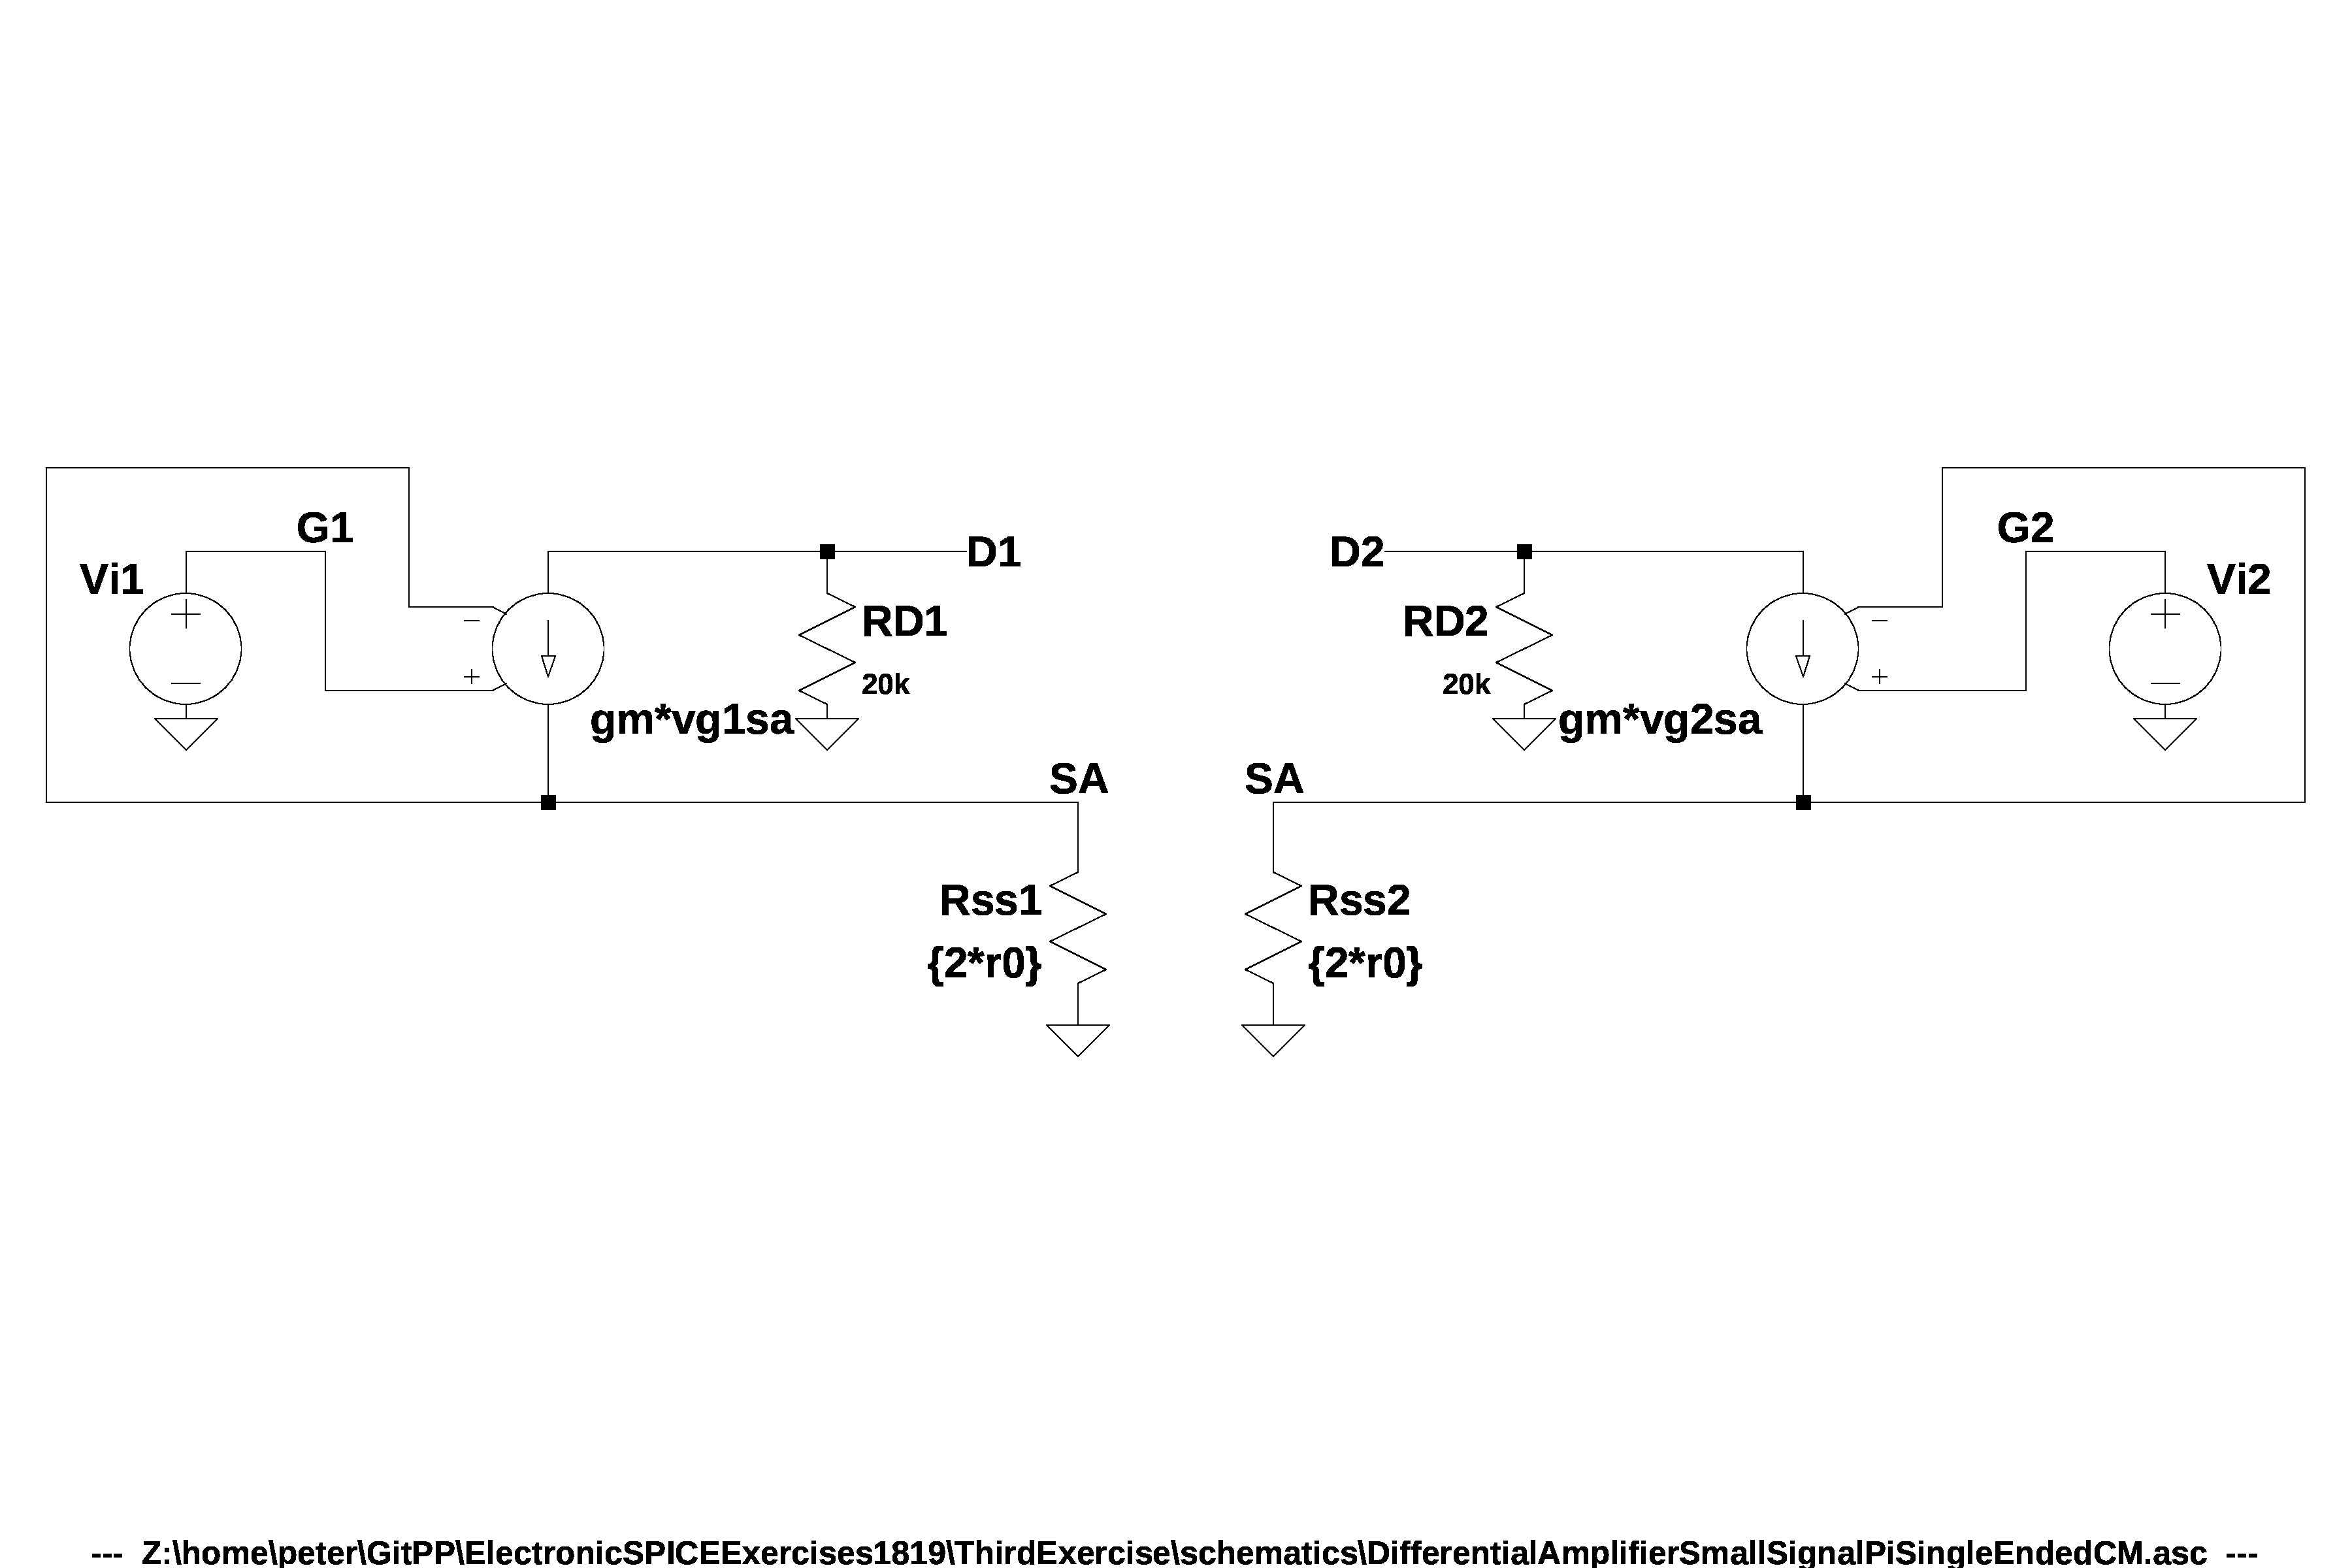
\includegraphics[width=12cm]{schematics/DifferentialAmplifier/SmallSignalPiSingleEndedCM.jpg}
  \caption{Small signal circuit single ended for a common mode signal.}
  \label{PiSingle2}
\end{figure}
Some useful equations for calculating the common mode gain are \ref{2r0} and \ref{VG1SAcm}.\\
\begin{align}
V_{i1} = V_{i2} = V_{i_{CM}} \label{vcm}\\
R_{ss_1} = R_{ss_2} = 2 r_0 \label{2r0}\\
V_{G_1S_A} = V_{G_2S_A}
\end{align}
\begin{align}
-V_{i_1} + V_{G_1S_A} + g_m V_{G_1S_A} R_{ss_1} &= 0\\
-V_{i_1} + V_{G_1S_A} (1+g_m R_{ss_1}) &= 0\\
\implies V_{G_1S_A} &= \frac{V_{i_1}}{1+g_m R_{ss_1}}\\ \xRightarrow{(eq.: \ref{2r0})}
V_{G_1S_A} &= \frac{V_{i_1}}{1+2g_m r_0}\label{VG1SAcm}
\end{align}

In order to calculate de common mode gain, the common mode gain of the single ended circuit are calculated first:\\
\begin{align}
V_{D_1} &= -g_m R_{D_1}V_{G_1S_A}\\
V_{D_1} &= -g_m R_{D_1} \left(\frac{V_{i_1}}{1+2g_m r_0} \right)\\
V_{D_1} &= \frac{-g_m R_{D_1}}{1+2g_m r_0}V_{i_1}\\
\implies \frac{V_{D_1}}{V_{i1}} &= \frac{-g_m R_{D_1}}{1+2g_m r_0}\\
\xRightarrow{(eq.: \ref{RD} and \ref{vcm})} \frac{V_{D_1}}{V_{i_{CM}}} &= \frac{-g_m R_{D}}{1+2g_m r_0} = A_{CM_{single\cdot ended\cdot 1}} \simeq \frac{R_{D}}{2r_0}
\end{align}

\begin{align}
A_{CM_{single\cdot ended\cdot 1}} \simeq \frac{R_{D}}{2r_0} \quad \text{for } r_0 \gg 1
\end{align}

\begin{align}
\frac{V_{D_2}}{V_{i_{CM}}} = \frac{-g_m R_{D}}{1+2g_m r_0} = A_{CM_{single\cdot ended\cdot 2}}\\
\end{align}
\begin{align}
A_{CM_{single\cdot ended\cdot 2}} \simeq \frac{R_{D}}{2r_0} \quad \text{for } r_0 \gg 1
\end{align}

The common mode gain is:\\
\begin{align}
A_{CM} &= \frac{V_{D_2} - V_{D_1}}{V_{i_{CM}}}\\
&= A_{CM_{single\cdot ended\cdot 2}} -A_{CM_{single\cdot ended\cdot 1}} \\
&= \left(\frac{-g_m R_{D}}{1+2g_m r_0} \right) - \left(\frac{-g_m R_{D}}{1+2g_m r_0} \right)\\
&= 0
\end{align}

\subsubsection{Common mode gain with $\lambda_3 = 0$}
With $\lambda_3 = 0$, the $r_0$ of the MOSFET $M_3$ isn't finite.\\
So the common mode gain would be null but also the single ended gain.\par

\clearpage
\section{SPICE analysis}
\subsection{$R_D = 20k$}
\subsubsection{Operating Point on static conditions ($\lambda_3 = 0$)}
\lstinputlisting{netlist/DifferentialAmplifier/StaticConditions.cir}
\lstinputlisting{netlist/DifferentialAmplifier/StaticConditions.op}

\subsubsection{Operating Point - common mode signals}
\lstinputlisting{netlist/DifferentialAmplifier/VCM.cir}
\lstinputlisting{netlist/DifferentialAmplifier/VCM.op}

\subsubsection{Operating Point - differential signals}
\lstinputlisting{netlist/DifferentialAmplifier/VID.cir}
\lstinputlisting{netlist/DifferentialAmplifier/VID.op}

\subsection{$R_D = 1097752/100$}
\subsubsection{Operating Point on static conditions ($\lambda_3 = 0$)}
\lstinputlisting{netlist/DifferentialAmplifier/StaticConditions100.cir}
\lstinputlisting{netlist/DifferentialAmplifier/StaticConditions100.op}

\subsubsection{Operating Point - common mode signals}
\lstinputlisting{netlist/DifferentialAmplifier/VCM100.cir}
\lstinputlisting{netlist/DifferentialAmplifier/VCM100.op}

\subsubsection{Operating Point - differential signals}
\lstinputlisting{netlist/DifferentialAmplifier/VID100.cir}
\lstinputlisting{netlist/DifferentialAmplifier/VID100.op}

\subsection{$R_D = 1097752/1000$}
\subsubsection{Operating Point on static conditions ($\lambda_3 = 0$)}
\lstinputlisting{netlist/DifferentialAmplifier/StaticConditions1000.cir}
\lstinputlisting{netlist/DifferentialAmplifier/StaticConditions1000.op}

\subsubsection{Operating Point - common mode signals}
\lstinputlisting{netlist/DifferentialAmplifier/VCM1000.cir}
\lstinputlisting{netlist/DifferentialAmplifier/VCM1000.op}

\subsubsection{Operating Point - differential signals}
\lstinputlisting{netlist/DifferentialAmplifier/VID1000.cir}
\lstinputlisting{netlist/DifferentialAmplifier/VID1000.op}
